\begin{tikzpicture}
    \begin{scope}[x={(0mm,300mm)},y={(0mm,199mm)},line width=1pt,cap=round]
        \node[anchor=south west,inner sep=0mm] at (0mm,0mm) {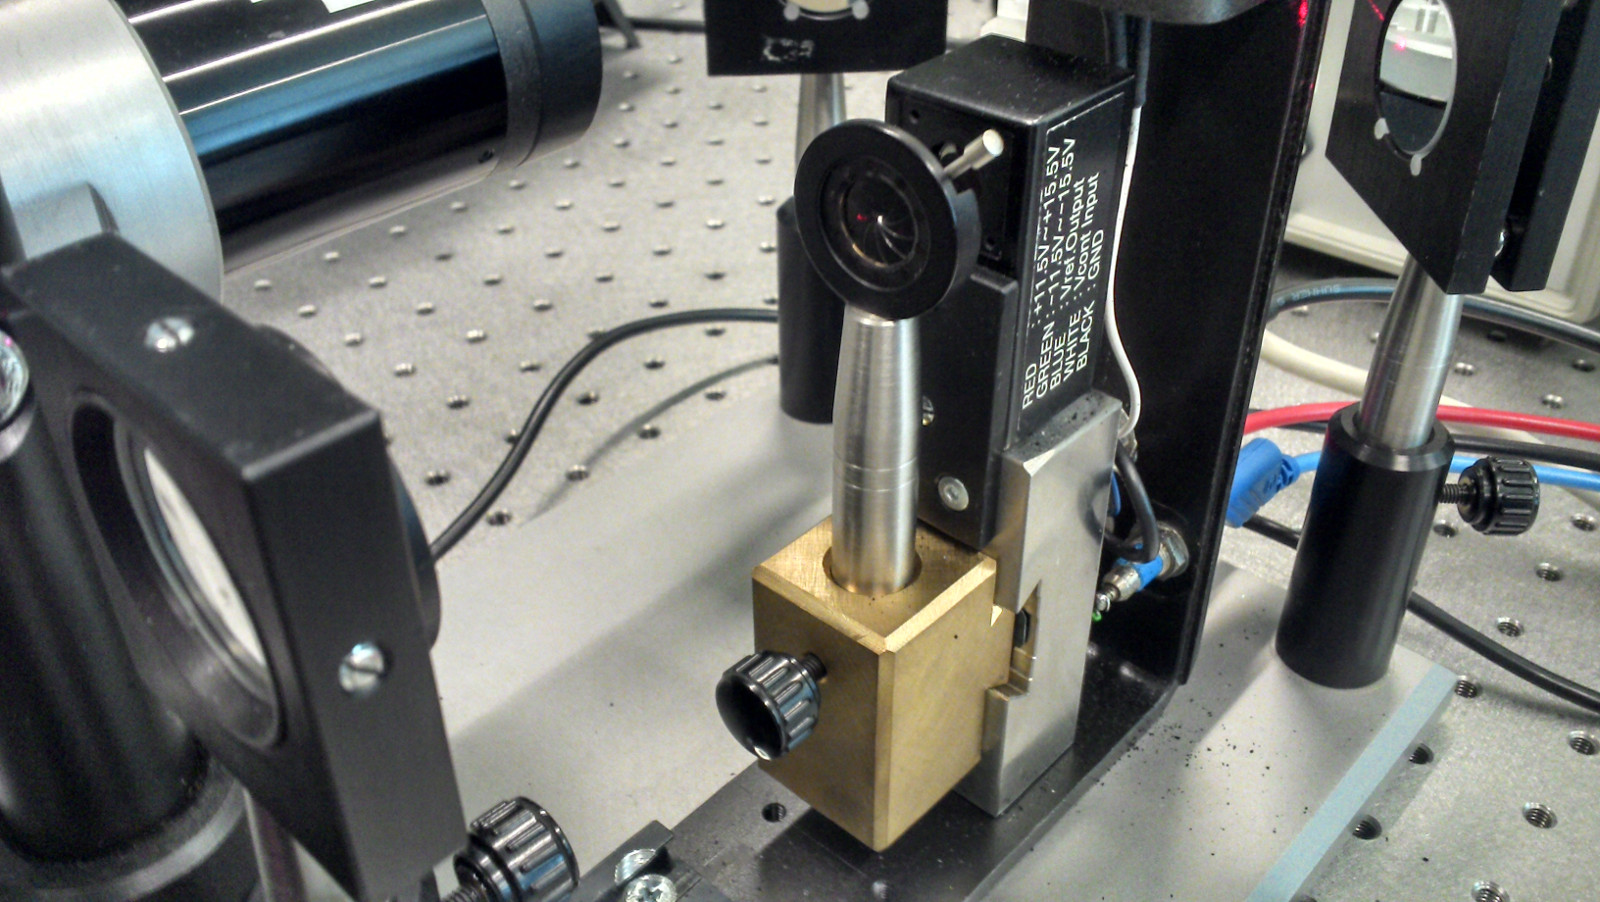
\includegraphics[width=300mm]{images/blende.jpeg}};

        %\draw[cyan] (210mm,80mm) -- (234mm,80mm);
        %\node[white] at (250mm,80mm) {\Large{\parbox{30mm}{\raggedright Geh\"ause mit \\Photomultiplier,\\ Blende und Linse $L_2$}}};
    \end{scope}
\end{tikzpicture}
